\chapter{Economic aspect of Operating Systems }
\label{chap:Economic_aspekt_of_Operating_Systems}


\section{Introduction}

In this section the relevance of Operating Systems in our Economic will be discussed. The importance of Operating Systems in our daily life is not always obvious.
The Operating System is the most important software on a computer. It manages the computer's memory, processes, and all of its software and hardware. 
With the rising amount Digitlization, the Operating System is also becoming more important than ever.

To get an over view on what an Operating System is, please refer to Chapter \ref{sec:WhatIsAnOs}.


\section{Operating System market share}

The Operating System Market is dominated by 4 major players. Android, Microsoft Windows, Linux and MacOS.
The market share if the Operting Systems is shown in Figure \ref{fig:Operating_Systems_Market_Share}. 

In the last years, the market share of Android has been increasing. This is due to the rising amount of smartphones and tablets.
Microsoft Windows is still the most used Operating System on Desktops and Laptops.

\begin{figure}[H]
    \centering
    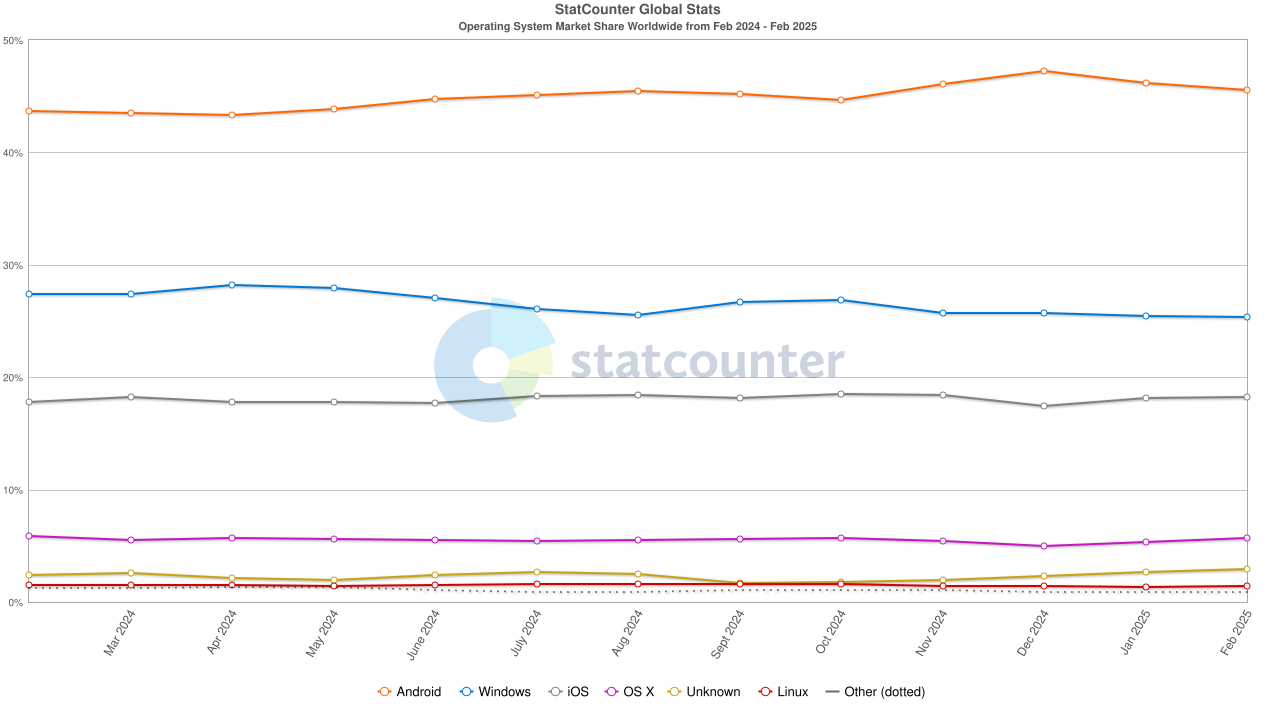
\includegraphics[width=0.8\textwidth]{figures/StatCounter-os_combined-ww-monthly-202402-202502.png}
    \caption{Operating Systems Market Share}
    \label{fig:Operating_Systems_Market_Share}
\end{figure}
\cite{OsMarketShare2}

The global market of Operating Systems is expected to reach \textdollar 48,18 billion at a CAGR of 1,9\% in 2026. 
\cite{OsMarketShare3}

\cite{OsMarketShare}
\cite{OsWikipedia}

\section{Operating Systems for Servers}

When looking at the Operating Systesms used for Webservers the market share looks very different.
The two main competitors are Microsoft and Red Hat. 

\begin{figure}[H]
    \centering
    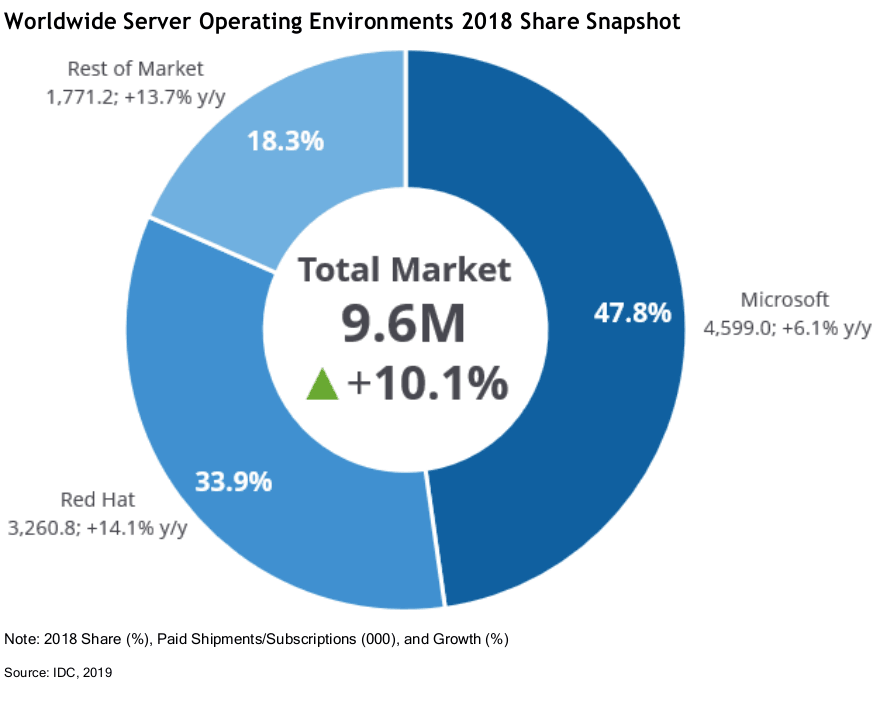
\includegraphics[width=0.8\textwidth]{figures/server-operating-system-market-share-2018.png}
    \caption{Operating Systems for Servers Market Share}
    \label{fig:Operating_Systems_for_Servers_Market_Share}
\end{figure}

As of 2018 Microsoft held 47,8\text{\%} of the Market while Red Hat held 33,9\text{\%}. 
The remaining 18,3\text{\%} of the market are shared by different competitors.   
\cite{SeverOsMarketShare}

\subsection{Market Volume}

Due to the rapid growth of the internet and related services, the market for servers and OS grew along side it. 
It's expected to grow to double of it current Volume by 2032. 




\author{Florian Prandstetter}